\section{Frameworks used in the Project}
\label{sec:frameworks}
In this section the different frameworks that have been in use in the project is presented.
The frameworks consists mainly of the development model, the different programming languages, the 
database and server tools, the Karotz API, the Android SDK and the IDE used for development.


\subsection{Programming Languages, Message Formats and File Formats}
The following section will comment on different programming languages, communication protocols and 
file formats used in the project.

\subsubsection{Eclipse IDE}
\label{sec:Eclipse}
Eclipse \cite{Eclipse} is a multi-language software development environment comprising an integrated development environment (IDE) and an extensible plug-in system. The source code is mostly written in Java. Eclipse may be used to develop applications in Java and, by means of various plug-ins, other programming languages including Ada, C, C++, Ruby, Python, and many others. Eclipse is owned by the Eclipse Foundation, a non-profit organization focusing on creating and maintaining a community for individuals and organizations who wish to collaborate on commercially-friendly open source software. 

\subsubsection{Java}

Java is a programming language developed by Sun Microsystems in 1995, and is licensed under the GNU General Public License. 
Java can be run on any Java Virtual Machine (JVM), which means that it can run on any platform. It is an object oriented language and is based upon classes.
According to TIOBE Software (2012)\cite{TIOBE}, it was ranked as the 2nd most popular programming language in the world.


\subsubsection{Android SDK}
The Android software development kit (SDK) \cite{AndroidSDK} includes a comprehensive set of development tools used when developing Android software. The kit includes an Emulator, documentation of the source code, sample code, tutorials and a debugger. Enhancements to Android's SDK go hand in hand with the overall Android platform development. The SDK will also support older versions of the Android platform, through downloading extra packages of source code, in case developers wish to target their application towards older devices. By building the project through the IDE the Android application is packaged in a format which may be distributed (.apk). 

\subsubsection{Android Developer Tools}
The Android Developer Tools (ADT) \cite{AndroidADT} is a plug in for Eclipse that provides a professional-grade development environment for building Android applications. The ADT makes it easier to use the functions and tools that the Android SDK provides, by giving access through the user interface of Eclipse.


\subsubsection{Javadoc}
Javadoc is a tool for documenting code. It is integrated in Eclipse IDE, and we will use it document our code. When we use code-completion in Eclipse, the Javadoc of the function selected is shown as it's description.  

\subsubsection{JavaScript}
Two parts of the project will make use of JavaScript. The settings page for doctors is web based and 
will use JavaScript for interactivity. The Karotz can be programmed in two ways; either through a web 
API on the server side or through stored JavaScript code. In order to maximize stability and power, 
the client hosted JavaScript technique will be used.

JavaScript is a multi-paradigm, weakly typed and dynamic language that is extensively used on the web 
today. The main application of JavaScript is to enhance interactivity on a web page through client-side 
interpretation of the code in a browser. It can be used for a number of purposes such as making something 
happen when a button is pressed, loading new data without refreshing the page and much more. Even 
though JavaScript is by far most commonly used on the web there are also applications of it in other 
areas. Examples of these kinds of implementations are Node.js\cite{nodejs}, a network application creation
platform for writing JavaScript code as a regular server-side program, and the Karotz API which we will be 
using.

\subsubsection{Karotz API}
The Karotz API is based on a Javascript engine. The API is downloadable from the 
Karotz's homepage and gives access to the Karotz's different functions such as changing the color 
of the LED light, playing prerecorded sounds, waving it's ears and registering contact with an RFID-chip. 

A full documentation of the API is given, however most of the example code is commented in French.

\subsection{Database}
Since the project team has decided to use a database to store information relevant to the systems, there
is a requirement to use a programming language for creating and maintaining, as well as accessing, the
database. Because of technical limitations in the Karotz explained further in Section \ref{sec:databaseAccessLayer}
we chose to split the database into to parts: the database itself, written and maintained in MySQL, and
a set of access modules written in PHP (PHP: Hypertext Preprocessor) and MySQL.

\subsubsection{MySQL and phpMyAdmin}
MySQL\cite{mysql} is the world's leading open source database. It offers all the tools necessary to implement
and maintain data records for a project such as ours. The advantage of being the biggest contender is that there
is a myriad of resources easily and freely available to MySQL developers on the Internet. MySQL is suitable
for our project because it is reliable, free and open source, and all the group members have previous experience
working with it.

PhpMyAdmin is a graphical MySQL manager that is installed on NTNU's MySQL server\cite{ntnuphpmyadmin}. It provides
an easy way to manipulate a MySQL database without having to write any SQL code. Figure \ref{fig:phpmyadmin} shows
a typical screen from phpMyAdmin, where one can edit, add rows, add information etc. directly within a GUI. Since
NTNU's servers are already integrated with the program, and we use NTNU's MySQL server for development,
phpMyAdmin will be used to administer the database efficiently.

\begin{figure}
	\begin{center}
		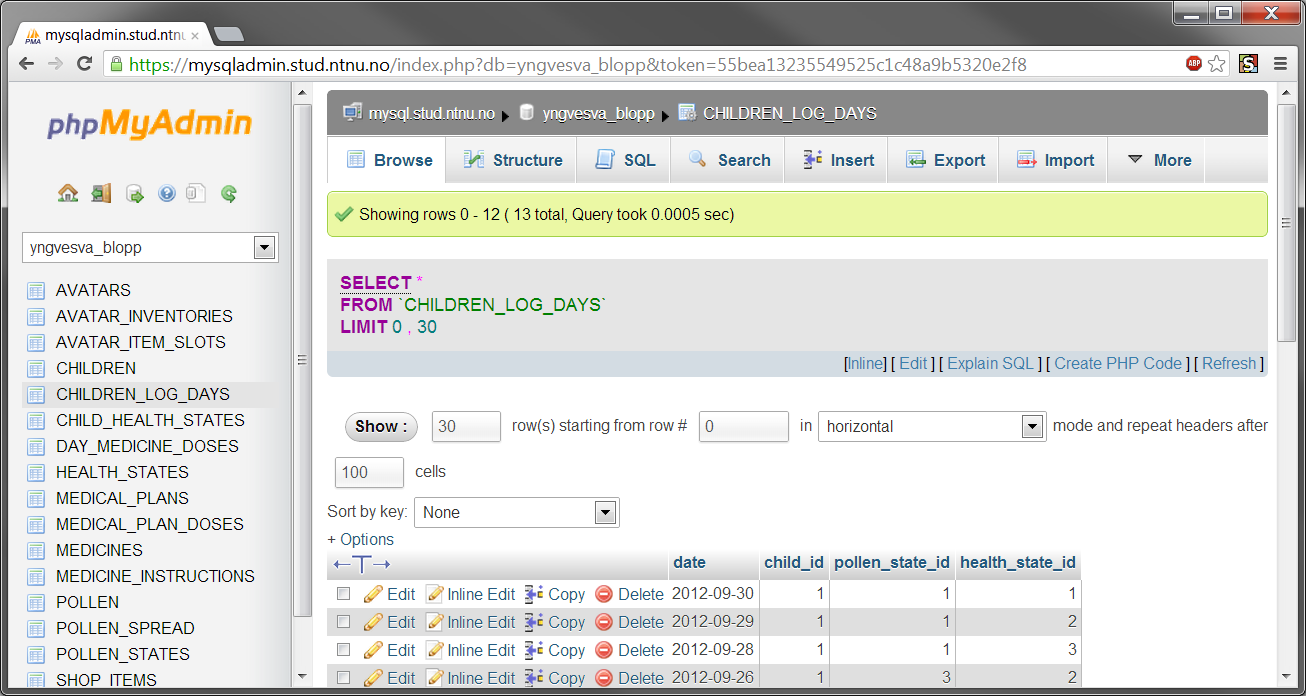
\includegraphics[width=17.5cm]{Pictures/Tools/PhpMyAdmin}
	\end{center}
	\caption{phpMyAdmin screenshot}
	\label{fig:phpmyadmin}
\end{figure}

\subsubsection{PHP}
PHP\cite{php} is a scripting language that is extensively used on the web because of its flexibility, ease of use
and popularity. It is mainly used for creating and editing HTML (HyperText Markup Language) pages server-side before sending to the client. In
our project, we used PHP to access the NTNU MySQL database from a web server located on a NTNU sub network(\url{http://folk.ntnu.no/}), 
and return a JSON file.

\subsubsection{JSON}
JSON\cite{json} is a format used for storing and sending data in a light, human-readable and easily parsable format.
It's based on JavaScript notation, but uses only a small subset of the JavaScript syntax; only strings, numbers, lists,
objects, booleans and the null value are included. We have used JSON for storing configuration data in the Karotz application, 
and for sending data between the PHP web access modules and the client applications.

\subsection{Extra Tools used in the Project}

The following section contains a description of the tools used for testing of the system, project and task 
management, team and customer collaboration, communication between participants. 
The tools chosen were chosen due to familiarity, making the learning curve as flat 
as possible. 

\subsubsection{Testing Tools}
This section describes tools used for performing unit tests, usability tests, and 
end-to-end tests.

\paragraph{HTTP Requests}
Postman\cite{postman} is a REST client for performing both basic and advanced HTTP requests to a
given URL. It is distributed as an extension for the \emph{Google Chrome} web browser. Postman keeps
a history of all sent requests, as well as an easy-to-understand interface for performing GET and
POST operations. Since the database was accessed through a web interface that used GET and POST methods,
it was natural to choose a REST client for the development process. Postman is also able to format
returned JSON, which was useful because the web access modules return JSON formatted data.
Figure \ref{fig:postman} shows a typical screen in Postman when performing a POST operation.

\subsubsection{Dropbox}
For file sharing between customer and the developer team, and the developer team 
between each other, we used Dropbox. Dropbox\cite{dropbox} is an online storage which 
allows sharing of folders and documents between invited partners. Dropbox is 
asynchronous, meaning only one person may edit a document at a time.

\subsubsection{Git}
To ensure that every team member was always up to date and no documentation was lost, 
version control systems were enforced. Git\cite{git} was used as a tool for version 
control. Git is a distributed source code management system, and was developed by Linus Torvalds in 2005. 
It comes with a lot of useful features like rollbacking to previous versions, file history and possibility to work on several branches, among others. 
The repository was hosted at Github (\url{http://github.com}). 

\subsubsection{Google Drive}
Google Drive (earlier Google Docs), is a file storage and synchronization service made by Google. Google Docs is now housed at Google Drive, and is 
a free web-based office suite. Google Docs allows several individuals to share and write the same document at the same time, and is ideal to write
simple documents concurrently.
Google Drive was used for writing agendas and status reports.


\begin{figure}
	\begin{center}
		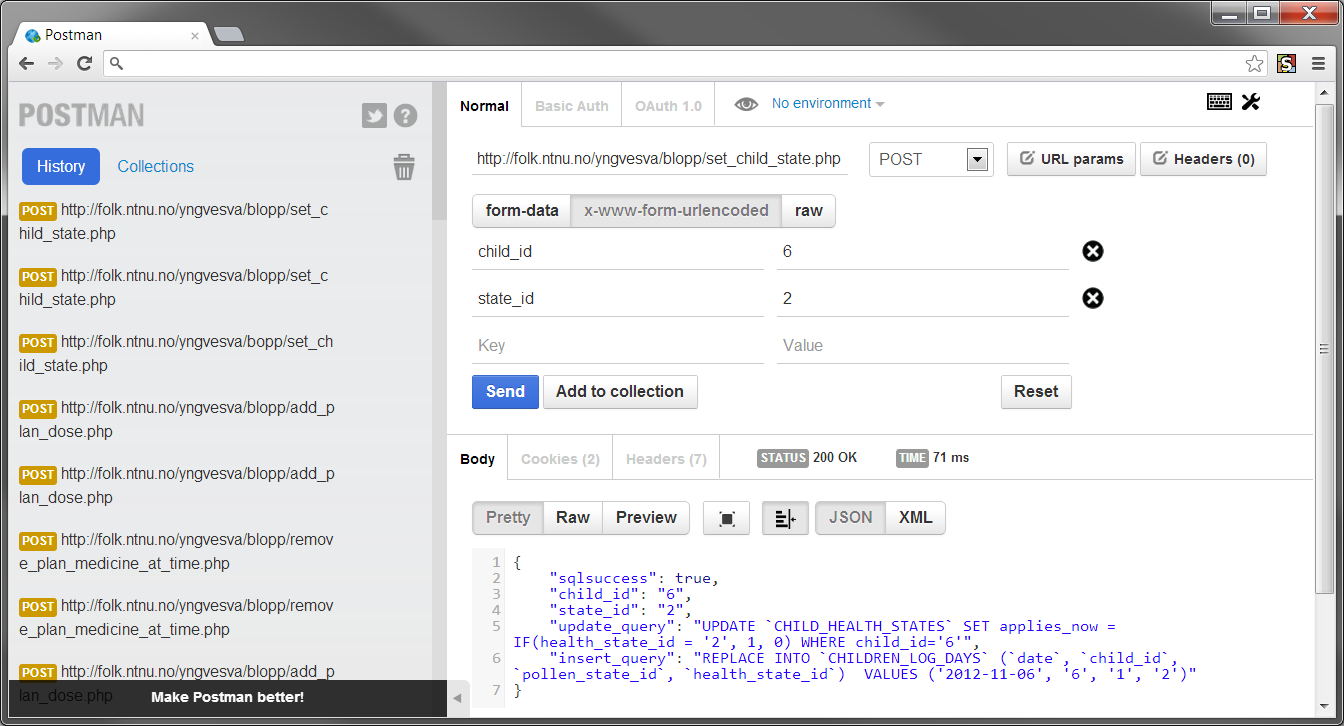
\includegraphics[width=17.5cm]{Pictures/Tools/Postman}
	\end{center}
	\caption{Postman screenshot}
	\label{fig:postman}
\end{figure}

% \subsection{Task Management, Collaboration and Communication Tools}
% The following section contains a description of the tools used for project and task 
% management, team and customer collaboration and communication between participants. 
% The tools chosen were chosen due to familiarity, making the learning curve as flat 
% as possible. 
% 
% For file sharing between customer and the developer team, and the developer team 
% between each other, we used Dropbox. Dropbox\cite{dropbox} is an only storage which 
% allows sharing of folders and documents between invited partners. Dropbox is 
% asynchronous, meaning only one person may edit a document at a time.
% 
% To ensure that every team member was always up to date and no documentation was lost, 
% version control systems were enforced. This way the information we made sure that an 
% online backup existed, in case of errors occuring. Git was used as a tool for version 
% control. 

\subsubsection{Task Management}
To ensure task management the team used AgileZen. AgileZen\cite{agilezen} is an online 
project management tool. You can add user stories, build a backlog and easily add 
tasks to each story. Unfortunately it is not perfect for projects using 
Scrum. AgileZen gives no simple way of keeping order of which task is to be done within a certain sprint. 
Their suggestion is using color coding of tasks, but this was not preferable.
There is also no way to assign a single task to a person, you may only sign epics/user stories to a user. Leaving no opportunity for showing that two people may work at the same use story at the same time. At a small project, such as ours this was at times a necessity, which AgileZen did not fulfill.
The team used AgileZen in order to keep the customer updated, while the team 
used Google Docs internally in order to keep track of tasks. 

\subsubsection{Mockup Tool}
For mockups the team chose Balsamiq Mockups. Balsamiq Mockups\cite{balsamiqmockups} is 
a tool designed for easing the collaboration between the GUI developers and the customer. 
The main advantage to Balsamiq Mockups is the way it ensures no one is too attached to the 
design. By making sketchy, low-fidelity frames it moves the focus of design conversations 
towards functionality. Balsamiq also has functionality for making click-through prototypes, 
which are very nice for demonstration purposes and usability testing. The team was also 
advised by the customer and the advisor to use Balsamiq Mockups.

\subsection{Design Principles}
Google\cite{androidguidelines}, who is developing the Android operating system has some design 
principles in order to help programmers make better applications. As Google 
states, quotation: "These design principles were developed by and for the Android User 
Experience Team to keep users' best interests in mind. Consider them as you apply your 
own creativity and design thinking. Deviate with purpose."

Many of these principles are guidelines to help the developers make more attractive 
and better applications, and some of them are rules, meant to follow without deviation. 
Google does not always state which is which, but refers to their slogan ``Don't be evil'', 
meaning developers should not try to scam, trick or hurt users through their applications.

The team as a group has read the design principles and would like to mention the ones that 
are most central for the applications we are making: 
\begin{description}
	\item[Real objects are more fun than buttons and menus.] The principles states that users should directly touch and manipulate objects, rather than 
	buttons and menus. This reduces the cognitive effort needed to perform a task while making 
	it more emotionally satisfying.
	\item[Let me make it mine.] People love to add personal touches because it helps them feel at home and in control. 
	Provide sensible, beautiful defaults, but also consider fun, optional customizations 
	that don't hinder primary tasks.
	\item[Keep it brief.] Use short phrases with simple words. People are likely to skip sentences if they're long.
	\item[Only show what I need when I need it.] People get overwhelmed when they see too much at once. Break tasks and information into 
	small, digestible chunks. Hide options that are not essential at the moment, and teach 
	people as they go.
\end{description}
